% !TEX encoding = UTF-8
% !TEX program = lualatex
\documentclass[tikz,border=10pt]{standalone}
\usepackage[UTF8]{ctex}
%\usepackage{luatexja-fontspec}
%\setCJKfamilyfont{Noto Sans CJK SC}
%%++++++++++++++++++++++++++++++++++++
\usepackage{tikz}
\usetikzlibrary{positioning}
\usetikzlibrary{shapes.geometric}% tikz node 形状的库
\usetikzlibrary{graphs,quotes,arrows.meta,graphs,shapes.misc}
\usetikzlibrary{graphdrawing}
\usegdlibrary{layered} 
\usegdlibrary[trees]
\usepackage{tikz-feynman}
\begin{document}

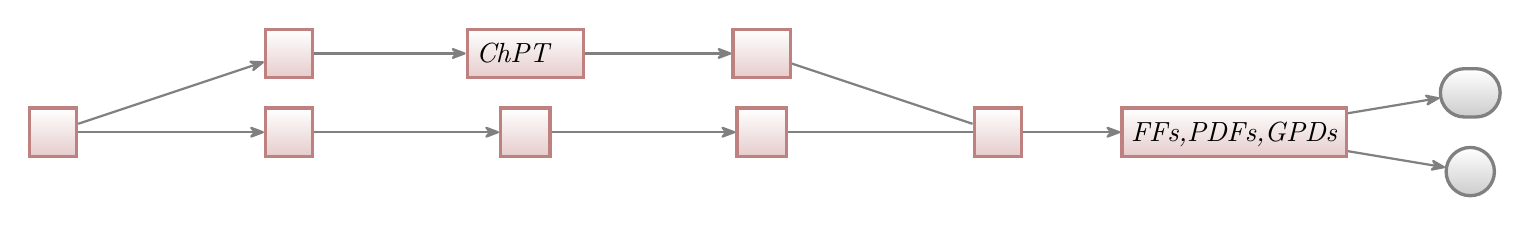
\begin{tikzpicture}[
	>={Stealth[round]}, black!50, text=black, thick,
	every new ->/.style = {shorten >=1pt},
	graphs/every graph/.style = {edges=rounded corners},
	nonterminal/.style = {
			rectangle, minimum size=6mm, very thick, draw=red!50!black!50, top color=white,
			bottom color=red!50!black!20, font=\itshape, text height=2ex,text depth=.5ex},
	terminal/.style = {
			rounded rectangle, minimum size=6mm, very thick, draw=black!50, top color=white,
			bottom color=black!20, font=\ttfamily, text height=2ex, text depth=.5ex}
	]
	%simple 的作用是,让一对node之间只能有一条连线,后发优先.
	\graph [tree layout,grow'=right, level distance=3cm]  {
	in/费曼图[nonterminal] -> {
        	coe/系数[nonterminal]->coech/ChPT 系数[nonterminal]->coeqf/夸克流系数[nonterminal] ,
                    int/圈积分[nonterminal]->"投影算符"[nonterminal]->结构函数[nonterminal],
    } -- /"组合"[nonterminal,grow'=down] -> out/"FFs,PDFs,GPDs"[nonterminal]-> {
        数值计算[terminal], 绘图[terminal]
        }
        };
\end{tikzpicture}

\end{document}


{
/ -> unsigned integer[nonterminal] -- p1 ->
"." [terminal] -- p2 -> digit[terminal] --
p3 -- p4 -- p5 -> E[terminal] -- q1 ->
"+"[terminal], q2, "-"[terminal]
}->	q3 -- /unsigned integer [nonterminal] -- p6 -> /;
p1 -> p4;
p3 ->p2;
p5 -> p6;
% 迫使这些 edge 平滑
q1 -- q2 -- q3;
};


